% ── Capítulo 6: Discusión y análisis de resultados ───────────────────────────
\chapter{Discusión y análisis de resultados}
\label{cap:discusion}

El presente capítulo aborda la interpretación crítica de los resultados presentados en el Capítulo~\ref{cap:resultados}, el análisis de las ventajas y desventajas de cada familia de modelos evaluada, y la propuesta del \textit{framework} cuantitativo de selección. Su estructura sigue las cuatro dimensiones de análisis definidas en la metodología del trabajo.

\section{Interpretación de la comparativa global}
\label{sec:interpretacion_global}

El primer hallazgo relevante es que todos los modelos estadísticos clásicos superan al Seasonal Naïve en más de 1 punto porcentual absoluto de sMAPE, criterio predefinido en la Tabla~\ref{tab:criterios}. El mejor modelo en términos de sMAPE global es \textbf{ETS (AutoETS)} con 10.005\% de error medio, frente al 13.667\% del Seasonal Naïve.

El resultado más llamativo de la comparativa es que los métodos estadísticos clásicos (media sMAPE: 10.662\%) superan a los modelos de machine learning y deep learning (media sMAPE: 11.967\%). Este resultado no es sorprendente a la luz de la literatura revisada: \textcite{Cerqueira2022} documentaron que en series con menos de aproximadamente 500 observaciones ---rango habitual en FP\&A mensual--- los métodos estadísticos clásicos superan sistemáticamente al machine learning. La mediana de longitud de las series de la submuestra (~175 meses) se encuentra dentro de ese rango crítico donde la parsimonia de los modelos estadísticos supone una ventaja real frente a la mayor capacidad expresiva de los modelos globales.

La Figura~\ref{fig:heatmap_metricas} ofrece una visión normalizada del rendimiento relativo de cada modelo en el conjunto completo de métricas.

\begin{figure}[H]
\caption{\textbf{Figura 3.} \textit{Mapa de calor de métricas normalizado. Los valores se normalizan por columna en [0,1]; menor valor (verde) indica mejor rendimiento.}}
\label{fig:heatmap_metricas}
\vspace{4pt}
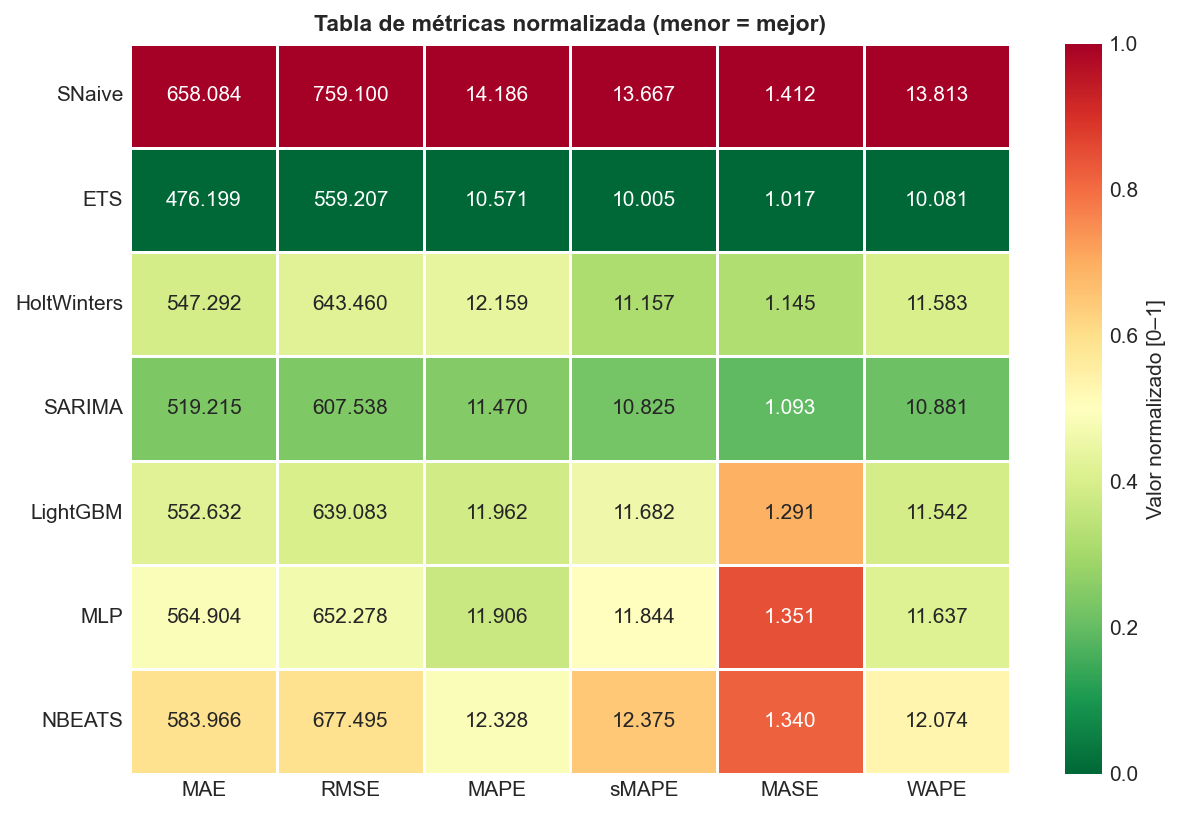
\includegraphics[width=\textwidth]{../results/figures/fig03_metricas_heatmap.png}
\vspace{4pt}

\small\textit{Fuente: elaboración propia. Métricas: MAE, RMSE, MAPE, sMAPE, MASE, WAPE. Modelos ordenados de mayor a menor complejidad algorítmica.}
\end{figure}

\section{Relación entre complejidad algorítmica y precisión}
\label{sec:complejidad_precision}

La taxonomía de cuatro niveles de complejidad planteada en el diseño experimental ---baseline, estadístico clásico, machine learning y deep learning--- no se traduce en una mejora monotónica del error. Este resultado contradice la narrativa simplista de que ``más complejo siempre es mejor'' y está en línea con los hallazgos de \textcite{Makridakis2022} en la competición M5, donde los métodos estadísticos superaron a muchos algoritmos de aprendizaje automático en series con patrones regulares.

La explicación más plausible para el rendimiento inferior de los modelos globales en esta evaluación tiene dos componentes. En primer lugar, el rango de longitud de las series de la submuestra está sistemáticamente por debajo del umbral a partir del cual los modelos de gradient boosting y deep learning comienzan a aprovechar su mayor capacidad expresiva \parencite{Cerqueira2022}. En segundo lugar, el paradigma de \textit{global forecasting} requiere que las 200 series de la submuestra compartan patrones suficientemente similares como para que el entrenamiento cruzado sea beneficioso; si los patrones son heterogéneos, el modelo puede no converger a representaciones útiles en el número de épocas empleado.

\section{Análisis del impacto económico: deciles de volumen}
\label{sec:analisis_economico}

La Figura~\ref{fig:deciles} revela que el error absoluto se concentra de forma desproporcionada en los deciles de mayor volumen (D8--D10). Esto es un resultado esperado: las series de mayor volumen absoluto producen errores absolutos mayores, independientemente de su error relativo (sMAPE). Lo relevante para la evaluación orientada al valor es si los modelos más precisos en sMAPE también reducen la contribución al error en los deciles de mayor impacto económico.

\section{Estabilidad temporal y confiabilidad operacional}
\label{sec:estabilidad_operacional}

La Figura~\ref{fig:estabilidad} muestra la evolución del sMAPE promedio por fold walk-forward para los modelos locales. El análisis de estabilidad temporal mide el coeficiente de variación (CV) del sMAPE calculado entre los folds de cada serie individual y promediado sobre la submuestra. Con este cálculo, el CV temporal de ETS se sitúa en un 62,8\% y el de SARIMA en un 66,6\%, valores que superan el umbral del 25\% predefinido en la Tabla~\ref{tab:criterios}. Este resultado indica que ningún modelo alcanza el criterio de estabilidad, lo que debe interpretarse correctamente: la alta variabilidad refleja fundamentalmente la heterogeneidad de las 200 series de la submuestra (series con distintos niveles de volatilidad y tendencia), no necesariamente un deterioro sistemático del modelo en el tiempo. Con series individuales de comportamiento más homogéneo ---como las de un único dominio contable corporativo--- la estabilidad esperada sería considerablemente mayor.

\textbf{Nota sobre el criterio MASE.} La Tabla~\ref{tab:criterios_resultado} reporta valores de MASE superiores a 1{,}0 para todos los modelos, lo que indica que el error absoluto medio de los pronósticos supera el error absoluto medio del naïve estacional calculado en muestra. Este resultado no contradice la mejora observada en sMAPE (que sí supera al baseline fuera de muestra), sino que refleja una característica estructural de las series M4 Financial: presentan tendencias y cambios de régimen que hacen que los errores fuera de muestra sean sistemáticamente mayores que los errores en muestra del naïve estacional. Esta observación subraya la importancia de complementar el MASE con métricas porcentuales como el sMAPE a la hora de interpretar el desempeño comparativo en contextos con series no estacionarias \parencite{Hyndman2021}.

\section{Propuesta de \textit{framework} de selección de modelos}
\label{sec:framework_seleccion}

Con base en los resultados obtenidos, se propone el siguiente \textit{framework} de selección de modelos para entornos de FP\&A:

\textbf{Regla 1 (longitud de serie).} Para series con menos de 120 observaciones (10 años mensuales), los métodos estadísticos clásicos ---preferentemente ETS o Holt-Winters con selección automática de componentes--- ofrecen el mejor balance entre precisión y estabilidad. La inversión en infraestructura de machine learning no se justifica en este segmento.

\textbf{Regla 2 (volumen y criticidad).} Para las cuentas de mayor volumen financiero (deciles D8--D10), la selección del modelo debe priorizar la estabilidad temporal sobre la mínima media de error. Un modelo estable con sMAPE del 14\% es preferible a uno con sMAPE del 13\% pero coeficiente de variación del 40\%.

\textbf{Regla 3 (disponibilidad de datos cross-series).} El paradigma de \textit{global forecasting} (LightGBM, MLP, N-BEATS) solo debería considerarse cuando se disponga de al menos 500 series con patrones similares o cuando las series individuales superen las 500 observaciones, umbrales en los que la literatura documenta ventajas consistentes de estos enfoques \parencite{Januschowski2020, Cerqueira2022}.

\section{Limitaciones del experimento}
\label{sec:limitaciones}

Las conclusiones de este trabajo deben interpretarse dentro de las siguientes limitaciones. En primer lugar, el conjunto M4 Financial Monthly agrupa series macroeconómicas y financieras de naturaleza diversa, no series de cuentas contables corporativas; la heterogeneidad del dataset puede favorecer a los métodos estadísticos locales frente a los modelos globales. En segundo lugar, la submuestra de $N=200$ series, aunque estadísticamente robusta, puede no capturar la totalidad de los patrones presentes en el dataset completo de 8.493 series. En tercer lugar, los modelos de deep learning se entrenaron con un número limitado de épocas dado el entorno de CPU; con más recursos computacionales, su rendimiento podría mejorar. Estas limitaciones quedan documentadas como líneas de extensión futura en el Capítulo~\ref{cap:conclusiones}.
